\begin{figure*}[t]  % [t]顶端；若想底部可用 [b] 并配合上面的包
    \centering
    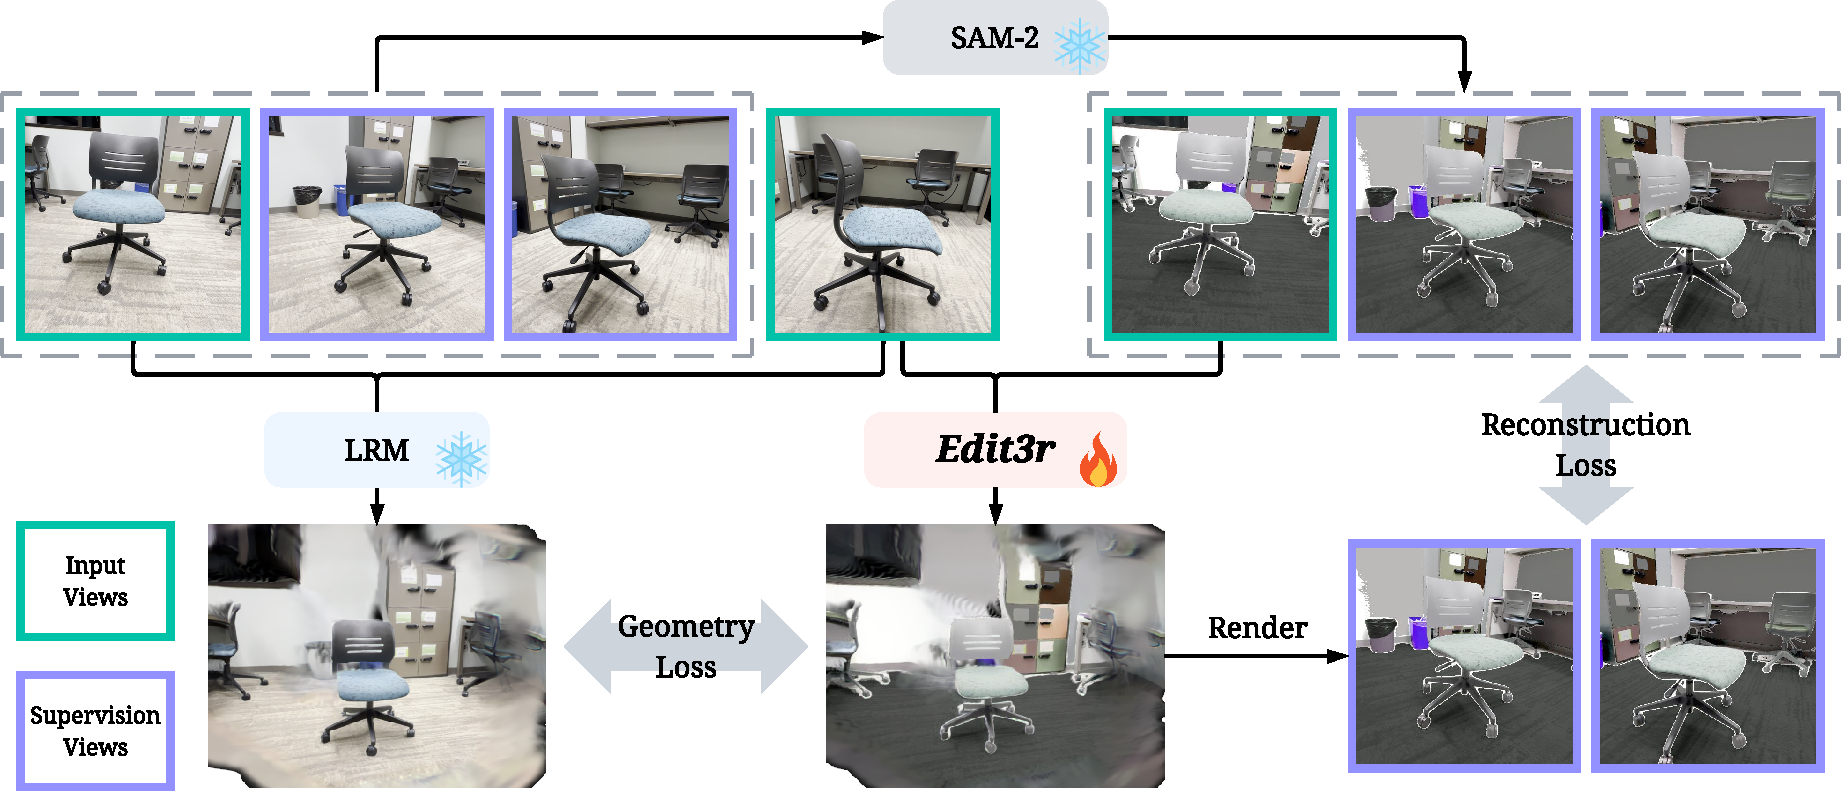
\includegraphics[width=\textwidth]{fig/pipeline_v4.pdf}
    \caption{\textbf{Training pipeline of \ourmethod.}
    Green-framed images are input views and purple-framed images are supervision views (ground-truth and rendered results).
    We first apply SAM2-based recoloring to both inputs and supervision views, then feed an asymmetric pair (one recolored view and one original view) into {\ourmethod} to predict a 3D Gaussian scene, which is rendered and supervised with reconstruction losses against the recolored supervision views (right).
    In parallel, a frozen LRM reconstructs the scene from the original inputs and provides 3D supervision via geometry losses that regularize {\ourmethod}’s Gaussian predictions in 3D space.}%绿色图片代表输入，紫色图片代表render结果和gt，我们会把输入和gt先用SAM2-based recoloring处理，用一张原图+一张recolor之后的图作为非对称数据输入给{\ourmethod},预测一个Gaussian，再把gaussian render出来跟我们recolor之后的GT去算Reconstruction Loss（图的右边部分）. 同时会用一个预训练好的LRM作为Supervision，通过Geometry Loss去约束{\ourmethod}在3D空间上的预测。（图的左边部分）
    \label{fig:pipeline}
    \vspace{-2mm}
\end{figure*}
\section{Method}
We propose a novel feed-forward framework for 3D scene editing. Given multi-view images and a text prompt, our method first applies 2D edits~\cite{ip2p, labs2025flux1kontextflowmatching, gpt4o} to the input images, and then reconstructs a 3D scene that is aligned with the text prompt, even when the edited images introduce multi-view inconsistencies. In contrast to optimization-based approaches~\cite{in2n, gaussctrl, gaussianeditor}, our pipeline enables real-time, instruction-guided editing by leveraging the efficient reconstruction capabilities of LRMs. Furthermore, {\ourmethod} is highly modular and can seamlessly integrate any 2D image editing technique, such as Instruct-Pix2Pix~\cite{ip2p} and FLUX~\cite{labs2025flux1kontextflowmatching}, thereby substantially enhancing the diversity and flexibility of the generated results.
% TODO整合3D Loss的叫法
\subsection{Preliminaries}
% Given a sequence of unposed images $I_v$ with corresponding camera intrinsics $k_v$, ${(I_v, k_v)}_{v=0}^{V-1}$, where $V$ denotes the number of input views, together with a text prompt $T$ for editing, our goal is to reconstruct a consistent 3D scene $S_T$ that is semantically aligned with the prompt.
Given a sequence of unposed images with corresponding camera intrinsics $\{(I_v, k_v)\}_{v=0}^{V-1}$ and an editing text prompt $T$, where $V$ is the number of input views, our goal is to reconstruct a geometrically consistent 3D scene $S_T$ that is semantically aligned with $T$.

During training, our pipeline takes one recolored image $(I'_0, k_0)$ and another original image $(I_1, k_1)$ from the unposed sequence as inputs to a feed-forward reconstruction model $f_{\theta}$ with learnable parameters $\theta$.
%
Instead of explicitly estimating camera poses or meshes, we approach reconstruction by lifting the unposed images into a canonical 3D Gaussian scene. Given views with unknown extrinsics, the network predicts a set of anisotropic Gaussian primitives in a fixed world frame. Each primitive encodes both geometry (location and shape) and appearance attributes (radiance and opacity).
%
Formally, we learn a function that maps image evidence to this representation:
\begin{equation*}
\mathcal{G} \;=\; f_{\theta}\!\left(\{(I'_0, k_0),(I_1, k_1)\}\right)
\end{equation*}
where $\mathcal{G}=\{(\mu_j,\Sigma_j,c_j,\alpha_j)\}_{j=0}^{V-1}$ denotes the predicted set of 3D Gaussians. $\mu\!\in\!\mathbb{R}^3$ is the center, $\Sigma\!\in\!\mathbb{R}^{3\times3}$ is the covariance, 
$c$ is a vector of spherical-harmonic color coefficients, and $\alpha$ is opacity.

\vspace{1mm}
\noindent\textbf{Pose-Free 3D Scene Reconstruction.}
Our approach adopts the pose-free 3D reconstruction framework of NoPoSplat~\cite{noposplat}. Given sparse unposed multi-view images, we embed the camera intrinsics for each view using a small MLP $\phi:\mathbb{R}^d \to \mathbb{R}^D$ concatenate these embeddings with the image token sequences to obtain the input tokens $z_v$:
\begin{equation*}
    z_v = \big[\,\text{img\_tokens}(I_v) \oplus \phi(k_v)\,\big],
\end{equation*}
A vision transformer (ViT)~\cite{vit} encoder with shared weights processes each view independently, taking $z_v$ as input and producing per-view features $f_v$ in a unified feature space. The set of features $\{f_v\}_{v=0}^{V-1}$ is then fused using a ViT decoder that leverages both self-attention and cross-view attention, enabling the model to resolve occlusions and appearance variations between views. This decoder outputs fused features $\{f_{fused}\}_{v=0}^{V-1}$, which are subsequently passed to two lightweight Gaussian heads.
%
Each Gaussian head contains two DPT-based~\cite{dust3r} predictors: one predicts the 3D centers of the Gaussians using only transformer features to ensure geometric stability; the other incorporates both the transformer features and RGB image shortcuts to estimate additional attributes, such as opacity, covariance, and low-order spherical harmonics for view-dependent color. For every input, the model produces a dense set of Gaussian primitives, which are concatenated in a canonical frame and rendered by standard 3D Gaussian splatting. The model is trained using photometric losses, eliminating the need for explicit pose input or pose-based warping and resulting in a pose-free, feed-forward pipeline.

\begin{figure}[t]  % [t] 顶端
    \centering
    \includegraphics[width=\linewidth]{fig/SAM2_recolor_v2.pdf}  
    \vspace{-2mm}
    \caption{Example of SAM2-based recoloring process.}
    \label{fig:SAM2-recolor}
    \vspace{-4mm}
\end{figure}

\subsection{SAM2-Based Recoloring} 
A key challenge in training our feed-forward 3D scene editing framework is the lack of multi-view consistent images paired with realistic edited inputs for supervision. To overcome this, we propose to approximate the editing task with recoloring. Specifically, we build upon SAM2~\cite{ravi2024sam} and design an object-aware segmentation and recoloring pipeline: the recoloring branch generates multi-view consistent supervision targets, while SAM2’s masks enable object-level appearance augmentations. These object-level augmentations play a crucial role in bridging the gap between our recolored training data and the edited images encountered at inference, ultimately enhancing the model’s generalization and performance. The overall data processing pipeline is illustrated in Fig.~\ref{fig:SAM2-recolor}.

\vspace{1mm}
\noindent\textbf{Object-Level Multi-Frame Segmentation via SAM2.} Given multi-view video frames $\{I_v\}_{v=0}^{V-1}$, we apply the automatic mask generator (AMG) from SAM2 on the first frame $I_0$ to automatically identify all candidate objects, without the need for manual prompts. Each AMG proposal $m$ provides a soft mask, area, stability score, predicted IoU, and a bounding box $b=(x, y, w, h)$, enabling efficient object selection and subsequent recoloring across views. 
%

We keep a proposal if it passes a deterministic multi-criterion filter:
(1) area $\ge A_{\min}$; 
(2) stability $\ge s_{\min}$; 
(3) predicted IoU $\ge q_{\min}$; 
(4) aspect ratio $w/h$ within $[r_{\min}, r_{\max}]$; 
(5) the box has at least $m_{\mathrm{edge}}$ pixels of margin to the image boundary. 
These parameter details are provided in the appendix. All retained instances are assigned persistent IDs and used to prompt the SAM2 video segmentation predictor (VSP) at $t{=}0$.

Next, we apply the VSP to the video sequence. For each frame $I_{v}$, the model identifies the set of active object IDs $O_v$ and corresponding per-object mask logits $Z_v^{(r)}$ which indicate foreground probabilities. Binary masks are obtained by thresholding the logits at zero, with pixels having logits greater than zero designated as foreground.
To mitigate identity drift, we only process a frame $v$ if its object-ID set $O_v$ sufficiently overlaps with that of the most recently processed frame $v^-$. Formally, we define the overlap ratio as $\frac{|O_v \cap O_{v^-}|}{\max(|O_v|, |O_{v^-}|)}$. If this ratio falls below 0.5, frame $I_v$ is skipped and excluded from all subsequent stages.
For all remaining (non-skipped) frames $v$ in the video, this stage produces per-object binary masks $\{M_v^{(r)}\}_{r \in O_v}$, which guide the subsequent region-wise recoloring process.

\vspace{1mm}
\noindent\textbf{Region-Wise Recoloring With Cross-View Consistency.}
We perform region-aware color augmentation by sequentially applying a composite color transform $\mathcal{C}_{\Theta_r}$ to each region. This transform consists of ColorJitter, gamma correction, PCA-based lighting offset, a fixed RGB-channel permutation, and optional grayscale conversion. The augmentation parameters $\Theta_r$ are sampled once per region and then reused across all frames and views to ensure consistent appearance.
%
When regions overlap, we re-normalize the per-pixel soft masks so that the mask weights sum to one over all overlapping regions (with a small $\varepsilon$ added to the denominator for numerical stability). The recolored image is then synthesized by soft blending:
\begin{equation*}
I_t' \;=\; 
\sum_{r\in\mathcal{R}} \hat{\alpha}_t^{(r)} \odot \mathcal{C}_{\Theta_r}(I_t)
\;+\;
\Big(1 - \sum_{r\in\mathcal{R}} \hat{\alpha}_t^{(r)}\Big) \odot I_t
\end{equation*}
Here, \(\odot\) denotes element-wise multiplication, and \(\hat{\alpha}_t^{(r)}\) is the per-pixel \emph{renormalized} mask weight for region \(r\); the remaining weight $1 - \sum{r\in\mathcal{R}} \hat{\alpha}_t^{(r)}$ at each pixel is assigned to the original image.
With a single region, this reduces to standard alpha blending between the transformed and original image.

\subsection{Loss Functions}
We train the model using both 2D supervision signals and 3D geometric constraints.  
%
For each view $v$, given the rendered prediction $\hat I_v$ produced by our model and the corresponding ground-truth image $I_v$, 
we optimize the model parameters by minimizing a weighted sum of three complementary loss terms across all views:
\begin{equation*}
\begin{split}
\label{eq:edit-loss}
\min_{\theta}\; \sum_{v=0}^{V-1}\Big[
&\mathcal{L}_{\text{CLIP}}(\hat I_v, I_v)
+\mathcal{L}_{\text{LPIPS}}(\hat I_v, I_v)
+\mathcal{L}_{\text{MSE}}(\hat I_v, I_v)
\Big] \\
&+\, \mathcal{L}_{\text{center}}
+\, \mathcal{L}_{\text{geom}}.
\end{split}
\end{equation*}
where the terms are weighted by their coefficients respectively
% $\lambda_{\text{clip}}$, $\lambda_{\text{lpips}}$, and $\lambda_{\text{mse}}$ .
%
The loss functions are defined as follows:  
a) a CLIP-based image-image loss $\mathcal{L}_{\text{CLIP}}(\hat I_v, I_v)$ that aligns the predictions with the targets in a semantic embedding space, providing a robust global supervision signal;  
b) a VGG-based perceptual loss $\mathcal{L}_{\text{LPIPS}}(\hat I_v, I_v)$ that enhances mid- and high-frequency details such as edges and textures, improving perceptual fidelity beyond pixel-level matching; and  
c) a low-frequency MSE loss $\mathcal{L}_{\text{MSE}}(\hat I_v, I_v)$ that enforces consistency in color, exposure, and illumination while remaining tolerant to small reprojection errors.

Beyond the 2D rendering losses, we introduce 3D regularization on the predicted Gaussian centers to stabilize the scene structure during editing.  
Because the editing applied to input images may distort depth cues and cause geometric inconsistencies across views, we leverage the pretrained LRM (NoPoSplat~\cite{noposplat}) to extract reference Gaussian centers $\mathcal{G}_{\text{ref}}$ from the unedited images.  
During training, the edited Gaussians $\mathcal{G}_{\text{edit}}$ are constrained to align with these reference centers using two complementary regularization terms.
%
%
First, a center-matching loss encourages each predicted Gaussian to remain close to its corresponding reference location, formulated as a Huber loss~\cite{huber1964robust} between the predicted and reference 3D centers:
\begin{equation*}
    \mathcal{L}_{\text{center}} = \mathrm{SmoothL1}(\hat{\boldsymbol{\mu}}, \boldsymbol{\mu}_{\text{ref}}).
\end{equation*}
This term preserves geometric fidelity to the original scene while permitting local deformations consistent with the applied edits.
%
Second, a multi-view consistency loss enforces structural coherence across different edited views by minimizing the pairwise Chamfer-$L_1$ distance between randomly sampled Gaussian centers from each view:
\begin{equation*}
\mathcal{L}_{\text{geom}} = \frac{1}{V(V-1)} 
\sum_{i<j}
\mathrm{Chamfer}_{L_1}(\hat{\boldsymbol{\mu}}_i,\hat{\boldsymbol{\mu}}_j)
\end{equation*}
This encourages a consistent 3D configuration across views, reducing depth-layer separation and suppressing “floating” artifacts caused by view-dependent misalignment.
% TODO: Show Example Images
Together, $\mathcal{L}_{\text{center}}$ anchors the edited scene to the base geometry learned by the pretrained reconstruction model, while $\mathcal{L}_{\text{geom}}$ encourages smooth geometric alignment across views.  
These 3D regularization terms complement the 2D perceptual and semantic losses by enforcing structural stability in the canonical Gaussian space, ensuring that scene edits remain spatially coherent and physically plausible.
%TODO：Add random drop

\begin{figure}[t]
    \centering
    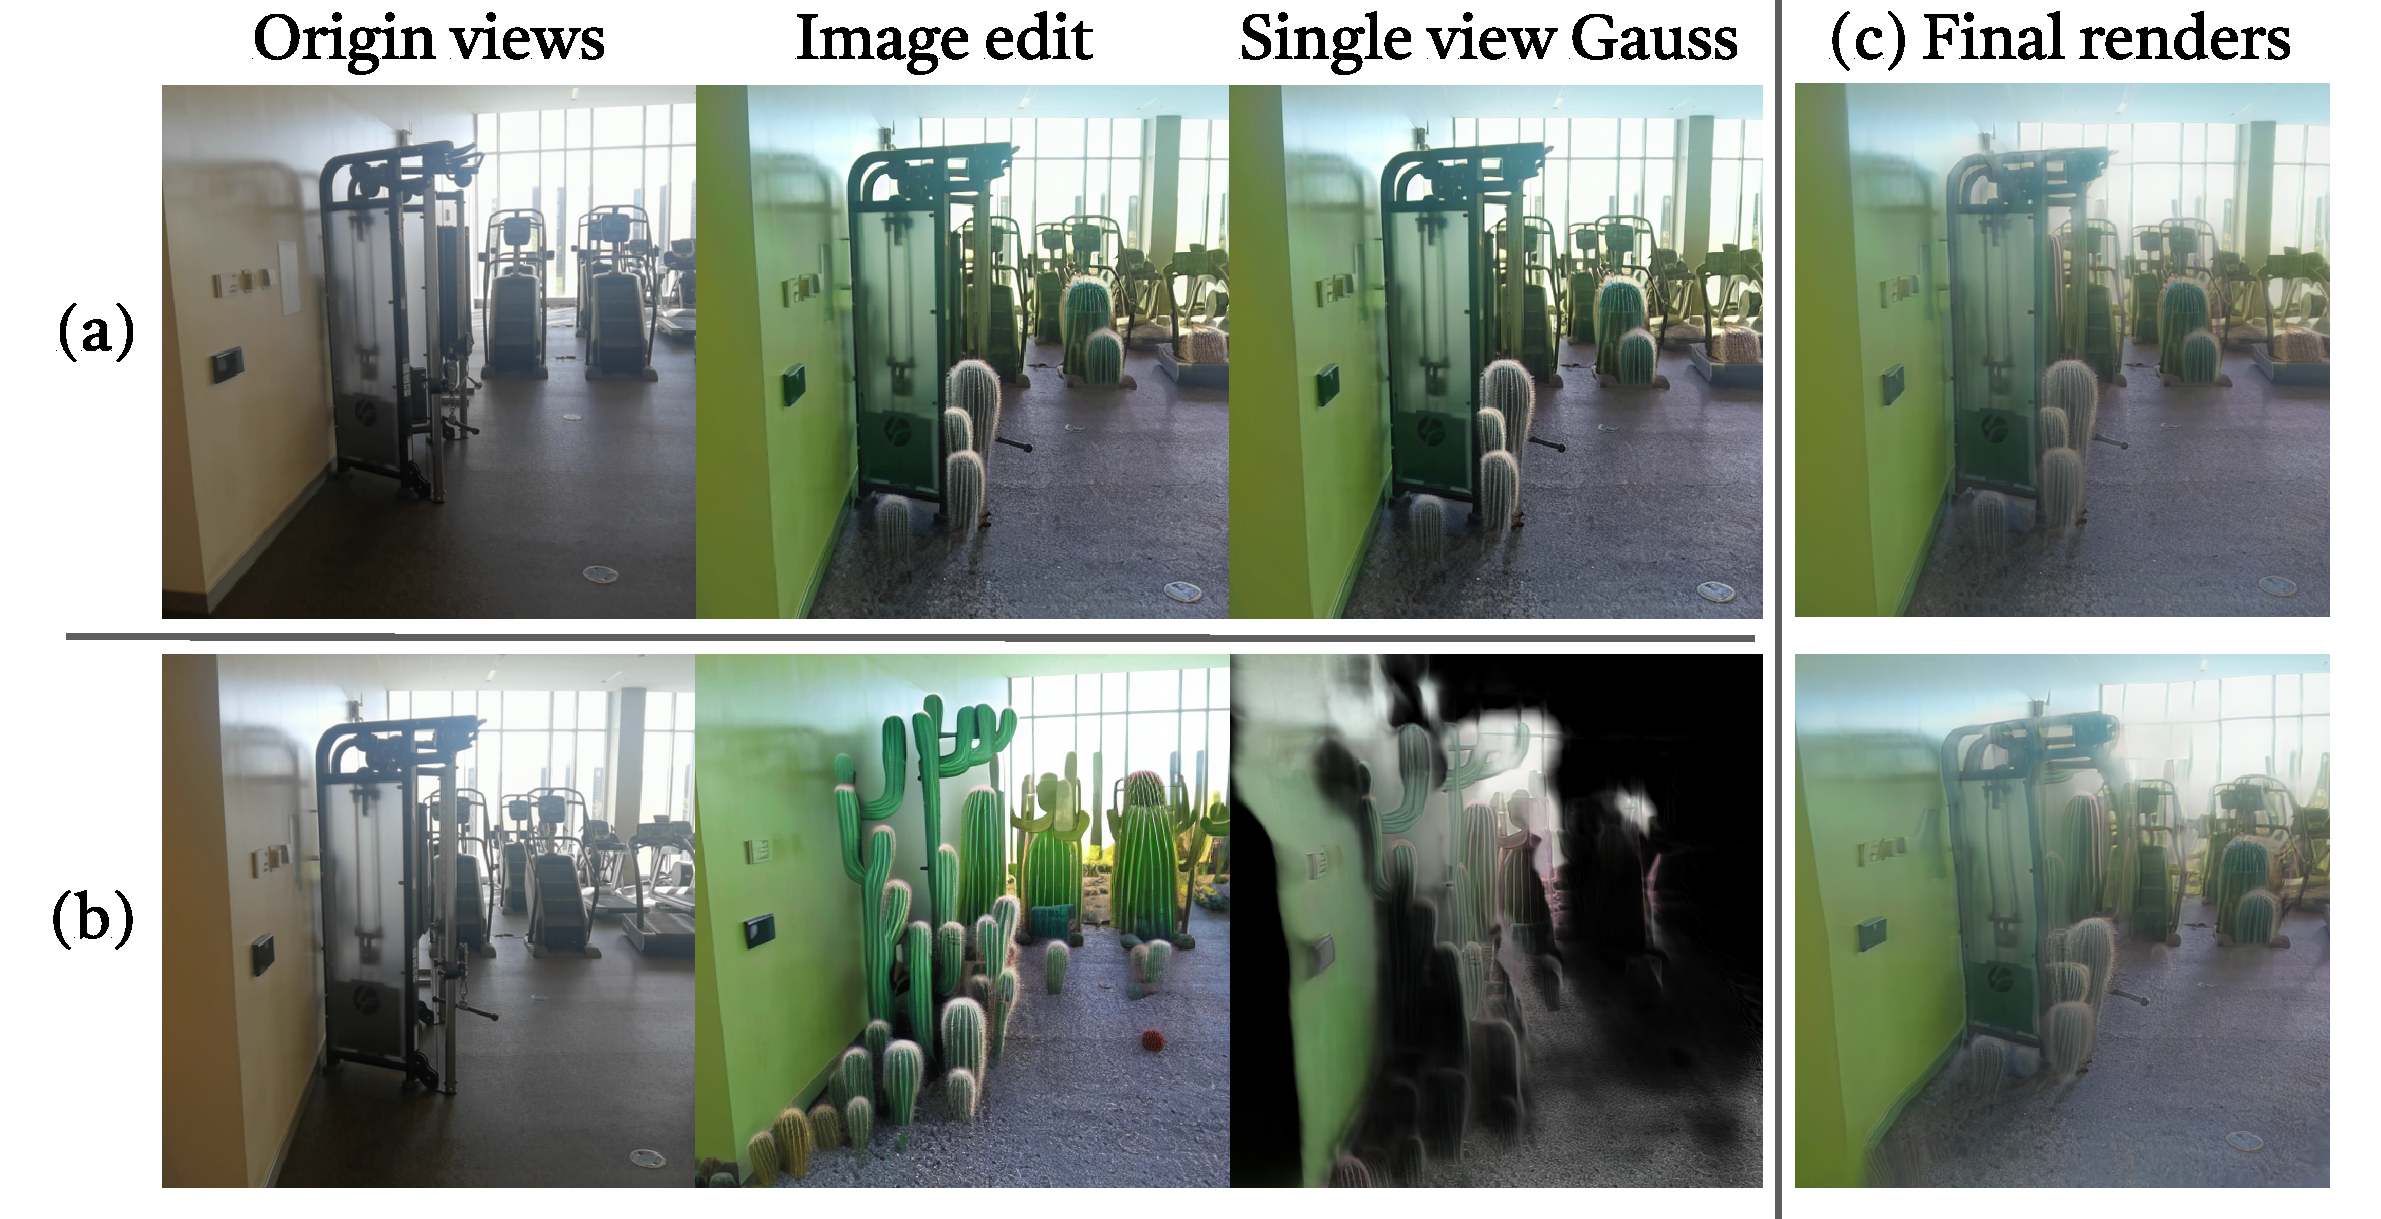
\includegraphics[width=\linewidth]{fig/edit_example_v2.pdf}  
    \caption{\textbf{Example of inference-time editing.}
    (a) First input view, its edited result, and the corresponding single-view Gaussian rendering.
    (b) Second input view, its edited result, and the corresponding single-view Gaussian rendering.
    (c) Final rendering obtained by combining Gaussians from both views. \textit{Prompt: Add a cactus garden.}}
    \label{fig:edit_example}
    \vspace{-2mm}
\end{figure}
\subsection{Inference}
Although our model is trained solely on recolored images, it generalizes effectively to images edited by various 2D editing methods~\cite{ip2p, labs2025flux1kontextflowmatching}.  
Unlike optimization-based pipelines that require iterative test-time fitting, inference in our system is fully feed-forward.  
Since the 2D editing stage operates independently from both the feed-forward reconstruction and the training procedure, our approach is highly flexible and can accommodate diverse image editing techniques~\cite{gpt4o, labs2025flux1kontextflowmatching, geminiteam2025geminifamilyhighlycapable}.  
For experiments and evaluations, we primarily employ commonly used IP2P~\cite{ip2p} as the 2D editor, while additional editors are included in ablation studies.  

As illustrated in Fig.~\ref{fig:teaser}, given a multi-view sequence \(\{I_v\}_{v=0}^{V-1}\) and a text instruction \(\mathcal{E}\), we first generate per-frame edited images \(\{I_v^\star\}_{v=0}^{V-1}\) with a 2D image editor.  
This differs from the training setup, where only the first frame is edited; at inference, all frames are edited to maximize cross-view evidence.  
We then perform a single feed-forward pass of {\ourmethod} to produce the edited 3D Gaussians and render novel views.
Fig.~\ref{fig:edit_example} provides a more concrete example: we visualize the Gaussians generated from the two input views separately in (a) and (b). 
Due to the inconsistency introduced by the 2D image editor, pixels in the second view can conflict with those in the first view; in these regions, the Gaussians from the second view automatically reduce their opacity to mitigate the conflict. 
Panel (c) shows the final rendering obtained by combining the Gaussians from both views, demonstrating view-consistent results.

\subsection{DL3DV-Edit-Bench}
\vspace{1mm}
\noindent\textbf{Motivation and Scope.}
Most existing 3D editing evaluations~\cite{in2n} either focus on single-object or toy scenes rather than full scene editing (\eg, limited context and occlusions), or rely on ad-hoc, privately curated data without a standardized protocol. This hampers fair comparison: methods differ in scene diversity, edit categories, and evaluation criteria. 
We therefore build \textbf{{\ourbench}} on top of the DL3DV~\cite{ling2023dl3dv10klargescalescenedataset} test split, covering diverse indoor/outdoor real scenes and four text-driven edit types: \emph{Add}, \emph{Remove}, \emph{Modify} (attribute/material/appearance), and \emph{Global} (style/exposure). The benchmark targets \emph{scene-level} editing under multi-view inputs and measures both edit effectiveness and cross-view consistency in realistic settings.

\vspace{1mm}
\noindent\textbf{Generation Pipeline.}
We start from the DL3DV test set and sample $20$ real-world scenes (indoor / outdoor). We first run Grounding-DINO~\cite{liu2024groundingdinomarryingdino} on all views to obtain object-level labels and region proposals. The per-scene image set and extracted labels are then fed to a large language model to synthesize candidate prompts for the four edit categories (Add / Remove / Modify / Global). 
We manually vet and keep $5$ valid prompts per scene, resulting in $100$ total edit instances. To ensure multi-view consistency during editing, we fix the 2D image editor, \emph{share} the same random seed and textual prompt across all views of a scene, and confine local edits with masks derived from the proposals. All editor hyperparameters (CFG, steps, strength schedule) are documented and kept constant unless otherwise stated.
